\section{Caja negra}
Una caja negra es un sistema que puede ser definido en terminos de sus entradas 
y salidas, sin conocimiento de su funcionamiento interno. Su implementación es 
opaca (negra). Se describirán los elementos del artefacto propuesto a 
continuación.

\textbf{Entradas:}
\begin{itemize}
  \item Flash Extend Density (FED) del satélite GOES-16.
\end{itemize}

\textbf{Habilitadores:}
\begin{itemize}
  \item Servidores de procesamiento.
  \item Sistema de alerta temprana.
\end{itemize}

\textbf{Restricciones:}
\begin{itemize}
  \item Tiempo de respuesta del satélite GOES-16.
  \item Tormentas eléctricas atípicas.
\end{itemize}


\textbf{Salidas:}
\begin{itemize}
  \item Probabilidad de ocurrencia de densidad de rayos (rayos/km$^2$).
\end{itemize}

\begin{figure}[H]
  \centering
  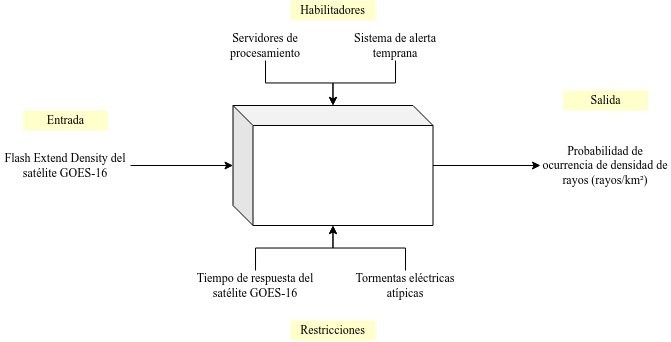
\includegraphics[width=14cm]{E_IMAGENES/4_Aporte/CajaNegra}
  \caption{
    Caja negra.
  }
  \label{fig:cajanegra}
\end{figure}